\subsubsection{CBus}
\index{CBus@\te{CBus} (package)}
\label{lib-cbus}

{\bf Package}

\begin{verbatim}
import CBus :: * ;
\end{verbatim}



{\bf Description}

The \te{CBus} package provides the interface, types and modules to
implement a configuration bus capability providing access to the
control and status registers in a given module hierarchy.  This
package  utilizes the
\te{ModuleCollect} package and functionality,  as described in section
\ref{package-modulecollect}.  The \te{ModuleCollect} package allows
items in addition to usual state elements and rules to be accumulated.
This is required to collect up the interfaces of the control status
registers included in a module and to add the associated logic and
ports required to allow them to be accessed via a configuration bus.

%For a more complete discussion of the \te{CBus}
%package, consult the configbus tutorial in the BSV/tutorials directory.



{\bf Types and Type Classes}

The type \te{CBusItem} defines the type of item to be collected by
\te{ModuleCollect}.   The items to be collected are the same as the
ifc which we will later expose, so we use a type alias:

\begin{libverbatim}
typedef CBus#(size_address, size_data) 
        CBusItem #(type size_address, type size_data);
\end{libverbatim}

The type \te{ModWithCBus} defines the type of module which is
collecting \te{CBusItem}s.  An ordinary module, one not collecting anything
other than state elements and rules, has the type \te{Module}.   Since
\te{CBusItem}s are
being collected, a  module type \te{ModWithCBus} is
defined.  When the module  type is not \te{Module}, 
the  type  must
be specified in square brackets immediately after the \te{module}
keyword in  the module definition. 

\begin{libverbatim}
typedef ModuleCollect#(CBusItem#(size_address, size_data), item) 
        ModWithCBus#(type size_address, type size_data, type item);
\end{libverbatim}



% typedef struct {
%    Bit#(size_address) a;
%    Bit#(size_address) o;
%    } CRAddr#(numeric type size_address) deriving(Bits, Eq);



{\bf Interface and Methods}
\index{CBus@\te{CBus} (interface)}
\index{IWithCBus@\te{IWithCBus} (interface)}

The \te{CBus} interface provides \te{read} and \te{write} methods to
access control status registers.  It is polymorphic in terms of the
size of the address bus (\te{size\_address}) and size of the data bus
(\te{size\_data}).  

%defines the interface for the configuration bus (the {\em back door} interface).  
\begin{center}  
\begin{tabular}{|p{.6 in}|p{4 in}|}
\hline
\multicolumn{2}{|c|}{\te{CBus} Interface}\\
\hline
Name &  Description\\
\hline
\hline 
&\\
\te{write}&Writes the \te{data} value to the register if and
only if the value of \te{addr} matches the address of the register.\\
\hline
&\\
\te{read}&Returns the value of the associated
register if and only if \te{addr} matches the register address.  In all
other cases the \te{read} method returns an \te{Invalid} value.\\
\hline
\end{tabular}
\end{center}


\begin{libverbatim}
interface CBus#(type size_address, type size_data);
   method Action write(Bit#(size_address) addr, Bit#(size_data) data);
   (* always_ready *)
   method ActionValue#(Bit#(size_data)) read(Bit#(size_address) addr);
endinterface

\end{libverbatim}

The \te{IWithCBus} interface combines the \te{CBus} interface with a
normal module interface.  It is defined as a structured
interface with two subinterfaces: \te{cbus\_ifc} (the associated
configuration bus interface) and \te{device\_ifc} (the associated
device interface).   It is polymorphic in terms of the type of the
configuation bus interface and the type of the device interface.  

%the device interface (the {\em front door} interface).

\begin{libverbatim}
interface IWithCBus#(type cbus_IFC, type device_IFC);
   interface cbus_IFC cbus_ifc;
   interface device_IFC device_ifc;
endinterface
\end{libverbatim}



{\bf Modules}

\index{collectCBusIFC@\te{collectCBusIFC} (module)}
\index[function]{CBus!collectCBusIFC}

The \te{collectCBusIFC} module 
takes as an argument a module with an \te{IWithCBus} interface, adds
the associated \te{CBus} interface to the current collection (using 
\te{addToCollection} from the \te{ModuleCollect} package), and returns
a module with  the normal interface.  Note that 
\te{collectCBusIFC} is of module type \te{ModWithCBus}.  

\begin{center}
\begin{tabular}{|p{1 in}|p{4.65 in}|}
\hline
&\\
\te{collectCBusIFC}& Adds the \te{CBus} to the collection and returns
a module with just the device interface.\\
\cline{2-2}
&\begin{libverbatim}
module [ModWithCBus#(size_address, size_data)] 
        collectCBusIFC#(Module#(IWithCBus#(
                        CBus#(size_address,size_data),i)) m)(i);
\end{libverbatim}
\\
\hline
\end{tabular}
\end{center}

\index{exposeCBusIFC@\te{exposeCBusIFC} (module)}
\index[function]{CBus!exposeCBusIFC}

The \te{exposeCBusIFC} module is used to create an \te{IWithCBus}
interface given a module with a normal interface and an associated
collection of \te{CBusItem}s.   This module takes as an argument a
module of type \te{ModWithCBus} and provides an interface of type
\te{IWithCBus}.   The \te{exposeCBusIFC} module exposes the
collected \te{CBusItem}s, processes them, and provides a new combined
interface.  This module is synthesizable, because it is of type \te{Module}.  

\begin{center}
\begin{tabular}{|p{1 in}|p{4.65 in}|}
\hline
&\\
\te{exposeCBusIFC}& A module wrapper that takes a module with a normal
interface, processes the collected CBusItems and provides an IWithCBus interface.\\
\cline{2-2}
&\begin{libverbatim}
module [Module] exposeCBusIFC#(ModWithCBus#(
            size_address, size_data, item) sm)
            (IWithCBus#(CBus#(size_address, size_data), item));
\end{libverbatim}
\\
\hline
\end{tabular}
\end{center}


The \te{CBus} package provides a set of module primitives each of which adds a
\te{CBus} interface to the collection and provides a normal \te{Reg}
interface from the local block point of view.  These modules are used
in designs where a normal register would be used, and can be read and
written to as registers  from within  the design.

\index{mkCBRegR@\te{mkCBRegR} (module)}
\index[function]{CBus!mkCBRegR}


\begin{center}
\begin{tabular}{|p{1 in}|p{4.65 in}|}
\hline
&\\
\te{mkCBRegR}&A wrapper to provide  a read only \te{CBus} interface
to the collection and a normal \te{Reg} interface to the local block.\\
\cline{2-2}
&\begin{libverbatim}
module [ModWithCBus#(size_address, size_data)] 
       mkCBRegR#(CRAddr#(size_address2) addr, r x)
                 (Reg#(r))
   provisos (Bits#(r, sr), Add#(k, sr, size_data), 
             Add#(ignore, size_address2, size_address));
\end{libverbatim}
\\
\hline
\end{tabular}
\end{center}
\index{mkCBRegRW@\te{mkCBRegRW} (module)}
\index[function]{CBus!mkCBRegRW}



\begin{center}
\begin{tabular}{|p{1 in}|p{4.65 in}|}
\hline
&\\
\te{mkCBRegRW}&A wrapper to provide  a read/write \te{CBus} interface
to the collection and a normal \te{Reg} interface to the local block.\\
\cline{2-2}
&\begin{libverbatim}
module [ModWithCBus#(size_address, size_data)] 
       mkCBRegRW#(CRAddr#(size_address2) addr, r x)
                 (Reg#(r))
   provisos (Bits#(r, sr), Add#(k, sr, size_data), 
             Add#(ignore, size_address2, size_address));
\end{libverbatim}
\\
\hline
\end{tabular}
\end{center}

\index{mkCBRegW@\te{mkCBRegW} (module)}
\index[function]{CBus!mkCBRegW}

\begin{center}
\begin{tabular}{|p{1 in}|p{4.65 in}|}
\hline
&\\
\te{mkCBRegW}&A wrapper to provide  a write only \te{CBus} interface
to the collection and a normal \te{Reg} interface to the local block.\\
\cline{2-2}
&\begin{libverbatim}
module [ModWithCBus#(size_address, size_data)] 
       mkCBRegW#(CRAddr#(size_address2) addr, r x)
                 (Reg#(r))
   provisos (Bits#(r, sr), Add#(k, sr, size_data), 
             Add#(ignore, size_address2, size_address));
\end{libverbatim}
\\
\hline
\end{tabular}
\end{center}



\index{mkCBRegRC@\te{mkCBRegRC} (module)}
\index[function]{CBus!mkCBRegRC}

\begin{center}
\begin{tabular}{|p{1 in}|p{4.65 in}|}
\hline
&\\
\te{mkCBRegRC}&A wrapper to provide  a read/clear  \te{CBus} interface
to the collection and a normal \te{Reg} interface to the local block.
This register can read from the config bus but the write is clear
mode; for each write bit a 1 means clear, while a 0 means don't clear. \\
\cline{2-2}
&\begin{libverbatim}
module [ModWithCBus#(size_address, size_data)] 
       mkCBRegRC#(CRAddr#(size_address2) addr, r x)
                 (Reg#(r))
   provisos (Bits#(r, sr), Add#(k, sr, size_data), 
             Add#(ignore, size_address2, size_address));
\end{libverbatim}
\\
\hline
\end{tabular}
\end{center}

\index{mkCBRegFile@\te{mkCBRegFile} (module)}
\index[function]{CBus!mkCBRegFile}

The \te{mkCBRegFile} module wrapper adds a \te{CBus} interface to the
collection and provides a \te{RegFile} interface to the design.  This
module is used in designs as a normal \te{RegFile} would be used.

\begin{center}
\begin{tabular}{|p{1 in}|p{4.65 in}|}
\hline
&\\
\te{mkCBRegFile}&A wrapper to provide  a normal \te{RegFile} interface and automatically
add the \te{CBus} interface to the collection. \\
\cline{2-2}
&\begin{libverbatim}
module [ModWithCBus#(size_address, size_data)] 
       mkCBRegFile#(Bit#(size_address) reg_addr, 
                    Bit#(size_address) size)
                    (RegFile#(Bit#(size_address), r))
   provisos (Bits#(r, sr), Add#(k, sr, size_data));
\end{libverbatim}
\\
\hline
\end{tabular}
\end{center}

{\bf Example}

Provided here is a simple example of a CBus implementation.  The
example is comprised of three packages: \te{CfgDefines},
\te{Block}, and \te{Tb}. The \te{CfgDefines} package contains
the definition for the configuration bus, \te{Block} is the design block,
and \te{Tb} is the testbench which executes the block.

The \te{Block} package contains the local design. As seen in Figure
 \ref{cbusreg},  the configuration bus registers look like a
 single field from the CBus (\te{cfgResetAddr, cfgStateAddr,
 cfgStatusAddr}), while  each field (\te{reset, init, cnt}, etc.) in 
 the configuration bus registers looks like a regular register from
 from the local block point of view. 

\begin{figure}[ht]
\begin{center}
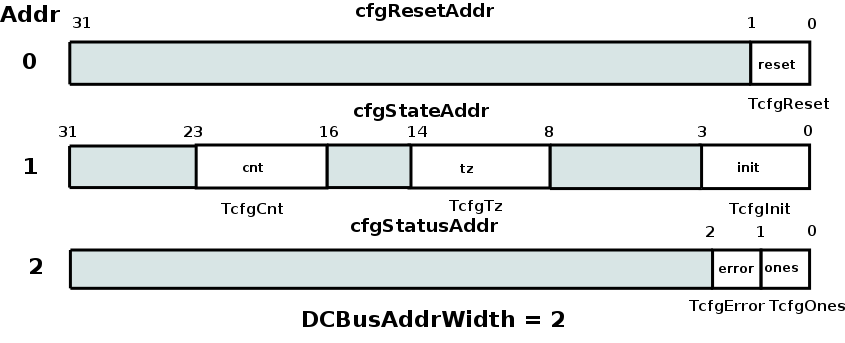
\includegraphics[width = 5 in]{LibFig/cbus1}
\caption{CBus Registers used in Block example}
\label{cbusreg}
\end{center}
\end{figure}

\begin{verbatim}
import CBus::*;       // this is a BSC library
import CfgDefines::*; // user defines - address,registers, etc

interface Block;
   // TODO: normally this block would have at least a few methods
   // Cbus interface is hidden, but it is there
endinterface

// In order to access the CBus at this parent, we need to expose the bus.   
// Only modules of type [Module] can be synthesized.
module [Module] mkBlock(IWithCBus#(DCBus, Block));
   let ifc <- exposeCBusIFC( mkBlockInternal );
   return ifc;
endmodule

// Within this module the CBus looks like normal Registers.
// This module can't be synthesized directly.
// How these registers are combined into CBus registers is 
// defined in the CfgDefines package.

module [DModWithCBus] mkBlockInternal( Block );
   // all registers are read/write from the local block point of view
   // config register interface types can be
   //   mkCBRegR  -> read only from config bus
   //   mkCBRegRW -> read/write from config bus
   //   mkCBRegW  -> write only from config bus
   //   mkCBRegRC -> read from config bus, write is clear mode
   //                i.e. for each bit a 1 means clear, 0 means don't clear
   // reset bit is write only from config bus
   // we presume that you use this bit to fire some local rules, etc
   Reg#(TCfgReset)  reg_reset_reset    <- mkCBRegW(cfg_reset_reset,    0 /* init val */);

   Reg#(TCfgInit)   reg_setup_init     <- mkCBRegRW(cfg_setup_init,    0 /* init val */);
   Reg#(TCfgTz)     reg_setup_tz       <- mkCBRegRW(cfg_setup_tz,      0 /* init val */);
   Reg#(TCfgCnt)    reg_setup_cnt      <- mkCBRegRW(cfg_setup_cnt,     1 /* init val */);

   Reg#(TCfgOnes)   reg_status_ones    <- mkCBRegRC(cfg_status_ones,   0 /* init val */);
   Reg#(TCfgError)  reg_status_error   <- mkCBRegRC(cfg_status_error,  0 /* init val */);

   // USER: you know have registers, so do whatever it is you do with registers :)
   // for instance
   rule bumpCounter ( reg_setup_cnt != unpack('1) );
      reg_setup_cnt <= reg_setup_cnt + 1;
   endrule

   rule watch4ones ( reg_setup_cnt == unpack('1) );
      reg_status_ones <= 1;
   endrule
endmodule
\end{verbatim}

The \te{CfgDefines} package contains the user defines describing how
the local registers are combined into the configuration bus.
\begin{verbatim}
package CfgDefines;
import CBus::*;

////////////////////////////////////////////////////////////////////////////////
/// basic defines
////////////////////////////////////////////////////////////////////////////////
// width of the address bus, it's easiest to use only the width of the bits needed
// but you may have other reasons for passing more bits around (even if some address
// bits are always 0)
typedef  2 DCBusAddrWidth;  // roof( log2( number_of_config_registers ) )

// the data bus width is probably defined in your spec
typedef 32 DCBusDataWidth;  // how wide is the data bus

////////////////////////////////////////////////////////////////////////////////
// Define the CBus
////////////////////////////////////////////////////////////////////////////////
typedef CBus#(  DCBusAddrWidth,DCBusDataWidth)          DCBus;
typedef CRAddr#(DCBusAddrWidth,DCBusDataWidth)          DCAddr;
typedef ModWithCBus#(DCBusAddrWidth, DCBusDataWidth, i) DModWithCBus#(type i);

////////////////////////////////////////////////////////////////////////////////
/// Configuration Register Types
////////////////////////////////////////////////////////////////////////////////
// these are configuration register from your design.  The basic
// idea is that you want to define types for each individual field
// and later on we specify which address and what offset bits these
// go to.  This means that config register address fields can 
// actually be split across modules if need be.
//
typedef bit      TCfgReset;

typedef Bit#(4)  TCfgInit;
typedef Bit#(6)  TCfgTz;
typedef UInt#(8) TCfgCnt;

typedef bit      TCfgOnes;
typedef bit      TCfgError;

////////////////////////////////////////////////////////////////////////////////
/// configuration bus addresses
////////////////////////////////////////////////////////////////////////////////
Bit#(DCBusAddrWidth) cfgResetAddr  = 0; // 
Bit#(DCBusAddrWidth) cfgStateAddr  = 1; // 
Bit#(DCBusAddrWidth) cfgStatusAddr = 2; // maybe you really want this to be 0,4,8 ???

////////////////////////////////////////////////////////////////////////////////
/// Configuration Register Locations
////////////////////////////////////////////////////////////////////////////////
// DCAddr is a structure with two fields
//     DCBusAddrWidth a ; // this is the address
//                        // this does a pure comparison
//     Bit#(n)        o ; // this is the offset that this register
//                        // starts reading and writting at

DCAddr cfg_reset_reset  = DCAddr {a: cfgResetAddr, o:  0};  // bits 0:0

DCAddr cfg_setup_init   = DCAddr {a: cfgStateAddr, o:  0};  // bits 0:0
DCAddr cfg_setup_tz     = DCAddr {a: cfgStateAddr, o:  4};  // bits 9:4
DCAddr cfg_setup_cnt    = DCAddr {a: cfgStateAddr, o: 16};  // bits 24:16

DCAddr cfg_status_ones  = DCAddr {a: cfgStatusAddr, o:  0};  // bits 0:0
DCAddr cfg_status_error = DCAddr {a: cfgStatusAddr, o:  1};  // bits 1:1

////////////////////////////////////////////////////////////////////////////////
///
////////////////////////////////////////////////////////////////////////////////
endpackage
\end{verbatim}

The \te{Tb} package executes the block.

\begin{verbatim}
import CBus::*;        // bsc library
import CfgDefines::*;  // address defines, etc
import Block::*;       // test block with cfg bus
import StmtFSM::*;     // just for creating a test sequence

(* synthesize *)
module mkTb ();
   // In order to access this cfg bus we need to use IWithCBus type
   IWithCBus#(DCBus,Block) dut <- mkBlock;
   
   Stmt test =
   seq
      // write the bits need to the proper address
      // generally this comes from software or some other packing scheme
      // you can, of course, create functions to pack up several fields
      // and drive that to bits of the correct width
      // For that matter, you could have your own shadow config registers
      // up here in the testbench to do the packing and unpacking for you
      dut.cbus_ifc.write( cfgResetAddr, unpack('1) );

      // put some ones in the status bits
      dut.cbus_ifc.write( cfgStateAddr, unpack('1) );
      
      // show that only the valid bits get written
      $display("TOP: state = %x at ", dut.cbus_ifc.read( cfgStateAddr ), $time);

      // clear out the bits
      dut.cbus_ifc.write( cfgStateAddr, 0 );

      // but the 'ones' bit was set when it saw all ones on the count
      // so read it to see that...
      $display("TOP: status = %x at ", dut.cbus_ifc.read( cfgStatusAddr ), $time);

      // now clear it
      dut.cbus_ifc.write( cfgStatusAddr, 1 );

      // see that it's clear
      $display("TOP: status = %x at ", dut.cbus_ifc.read( cfgStatusAddr ), $time);

      // and if we had other interface methods, that where not part of CBUS
      // we would access them via dut.device_ifc 
   endseq;
   mkAutoFSM( test );
endmodule
\end{verbatim}

